\chapter{To Tune or Not to Tune? \\ In Search of Optimal Configurations for Data Analytics}

\textbf{Reference:}~\url{https://dl.acm.org/doi/pdf/10.1145/3394486.3403299}

\textbf{Code:}~\url{https://github.com/ayat-khairy/tuneful-code}

\textbf{Keywords:} spark, configuration tuning, bayesian optimization

\section*{Какую задачу решают авторы?}

При разработке Spark приложений, разработчики не так часто занимаются вопросом подбора оптимальных параметров (конфигарации) для запуска приложения.

Это может приводить к различным последствиям, например, 
\begin{itemize}
    \item аллокация под приложение слишком большого числа ресурсов, в результате другим приложениям может нехватать ресурсов
    \item аллокация слишком маленького для задачи числа ресурсов, как следствие приложение работает слишком медленно или вообще не работает из-за нехватки ресурсов
\end{itemize}

Существуют инструменты для тюнинга конфигураций приложений, которые позволяют избежать подобных ситуаций.

(Тут должен быть блок про предыдущие решения и их недостатки, в работе упоминаются два инструмента: Opentuner\footnote{\url{http://opentuner.org}} и Gunther\footnote{\url{https://link.springer.com/chapter/10.1007/978-3-642-40047-6_42}})

Но им часто требуется большое количество (порядка 100) exploration запусков и ими не очень удобно пользоваться. \\

В статье авторы предлагают фрэймворк Tuneful, который интегрирован в экосистему Spark'a и позволяет относительно быстро тюнить конфигурации приложений.

\section*{Как решают}

На рисунке~\ref{fig:tuneful} показано как Tuneful интегрирован в Spark.

\begin{figure}[ht]
    \centering
    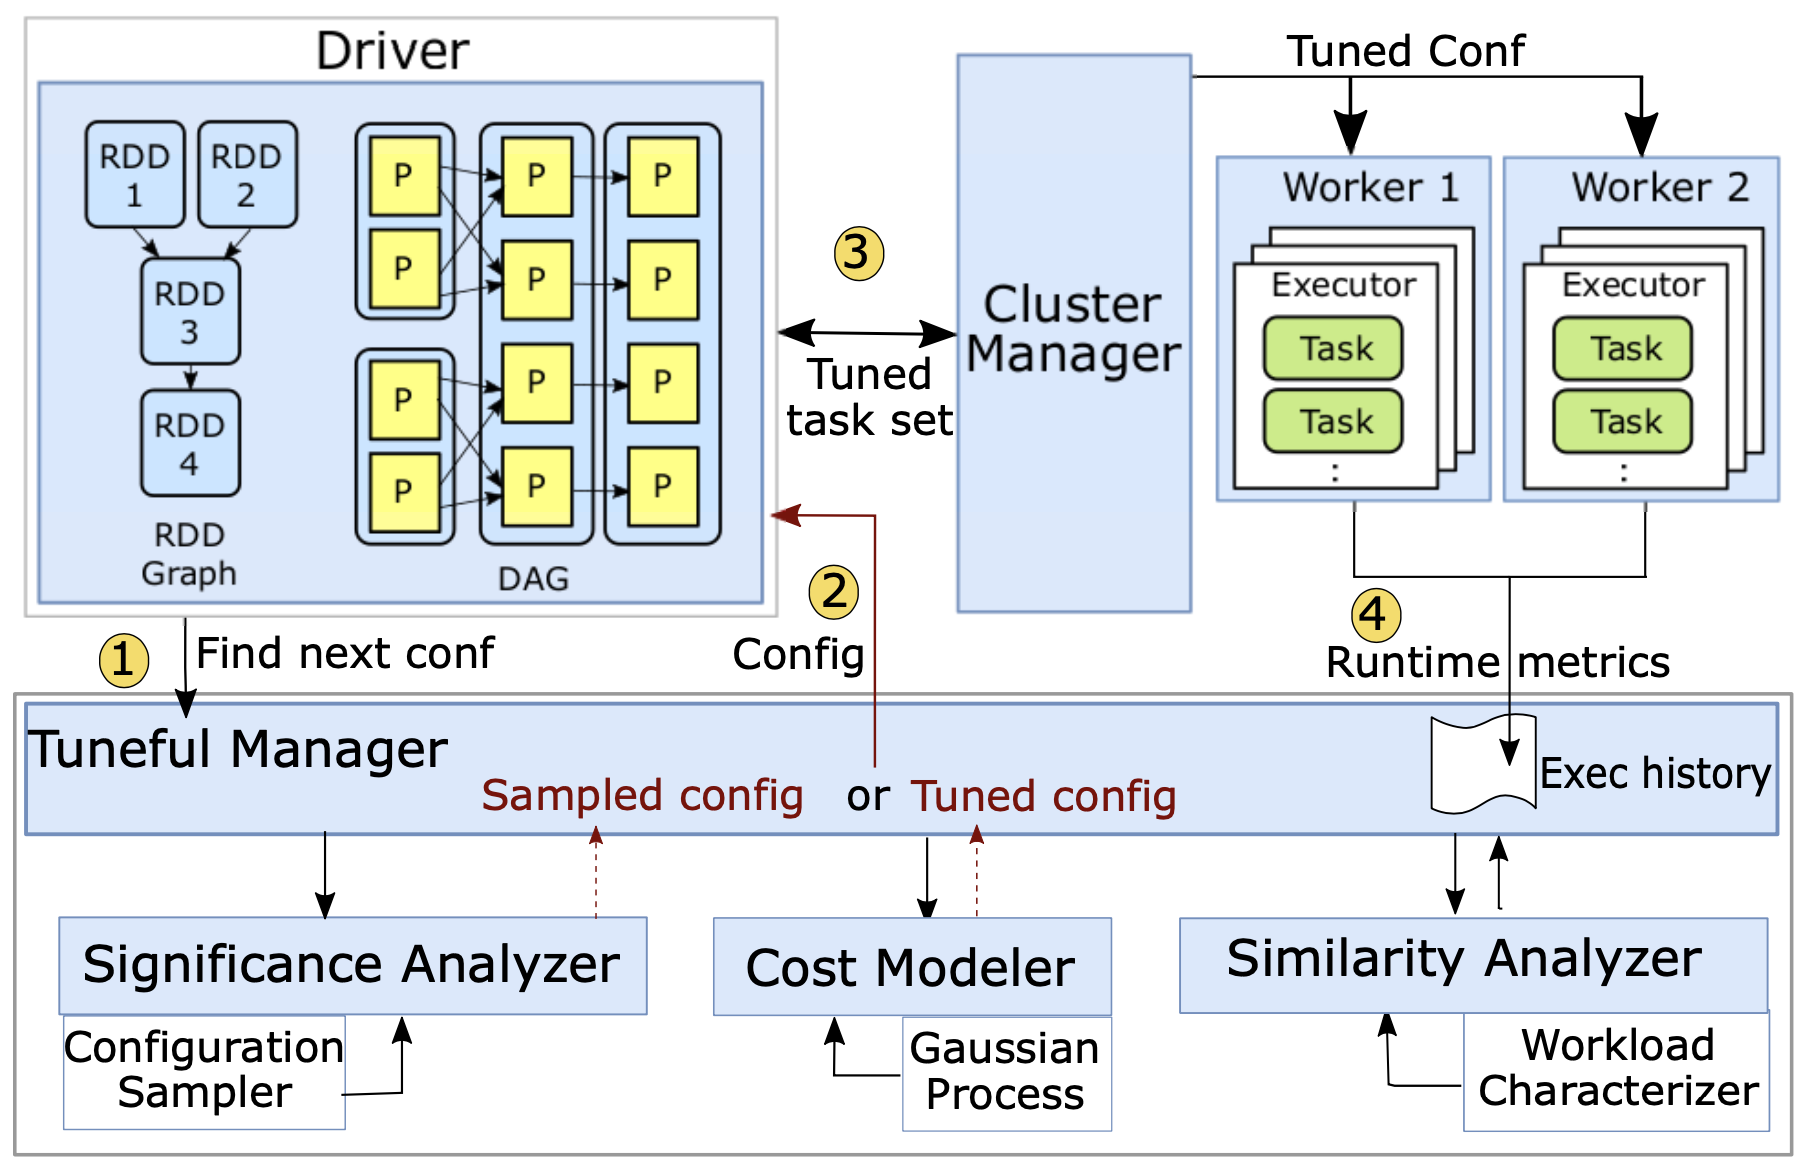
\includegraphics[width=0.7\linewidth]{images/tuneful.png}
    \caption{\footnotesize{Tuneful–Spark integration: (1) При запуске приложения, Driver запрашивает конфигурацию в Tuneful. (4) После завершения приложения, метрики (время работы, потребление ресурсов итд) отправляются в Tuneful для обновления модели оптимизации.}}
    \label{fig:tuneful}
\end{figure}

Tuneful состоит из трех основных компонент: Significance Analyzer, Cost Modeler и Similarity Analyzer. 

\newpage

Кратко работа Tuneful выглядит следующим образом:
\paragraph{Significance Analyzer} Также как и в большинстве фрэймворков для оптимизации гиперпараметров ML алгоритмов, процеcc оптимизации в Tuneful можно разбить на фазу поиска (exploration) и фазу использования лучшей из найденных конфигураций (exploitation).
    
В начале фазы поиска Significance Analyzer пытается выделить application-specific важные параметры --- запускает приложение с разными конфигурациями, чтобы понять, какие параметры сильнее всего влияют на время работы приложения.

\paragraph{Cost Modeler} После того как было выполнено достаточное количество exploration запусков (на практике требуется около 35), Cost Modeler использует информацию об exploration запусках и строит модель, которая позволяет по \textbf{конфигурации важных параметров} предскзывать время работы приложения (неважные параметры при этом остаются фиксированными).
    
Для построения модели Cost Modeler использует Гауссовские процессы.

Построенная модель используется для получения конфигурации для очередного запуска приложения.

После каждого очередного запуска приложения, Cost Modeler получает информацию о времени работы приложения и обновляет модель. \\

Когда Tuneful находит достаточно хорошую конфигурацию для приложения, процесс тюнинга останавлиявается и для последующих запусков используется найденная конфигурация.
    
\paragraph{Similarity Analyzer} Когда Tuneful используется уже продолжительное время (тюнил конфигурации для большого числа приложений), то при тюнинге параметров для нового приложения, Tuneful может использовать информацию о \textit{похожих} приложениях для более удачного старта процесса тюнинга.
    
Поиском похожих приложений занимается Similarity Analyzer.

Для того чтобы посчитать похожесть между приложениями, авторы описывают их с помощью большого количества метрик, которые собирают во время работы приложения.

На собранных метриках обучают autoencoder, для того чтобы для приложения получить описание в виде вектора меньшей размерности.

\subsection*{Experiments}

Авторы проводят большое количество экспериментов для того чтобы оценить качество предложенного фрэймворка. \\

Для экспериментов используют два кластера: первый из 20 машин и второй из 4х.

В качестве приложений для оптимизации авторы выбрали 5 довольно сильно отличающихся друг от друга приложений. 

В качестве бэйслайнов авторы используют Random Search, Opentuner и Gunther. \\

Авторы показывают, что Tuneful позволяет примерно в 3 раза быстрее найти хорошие конфигурации, и что использование Similarity Analyzer'a позволяет в 3 раза ускорить тюнинг для новых приложений.

\section*{Выводы}

\dbox{\textbf{Key Takeaways:}
\begin{enumerate}
    \item Если приложение запускается суммарно меньше 100 раз, то нет смысла пытаться его тюнить используя специальные фрэймворки из-за большого числа exploration запусков.
    \item Если речь идет о приложении, которое, например, запускается по крону каждый день, то оно идеально подходит для тюнинга конфигурации, но нужно быть готовым к тому, что в течении первых 30 запусков почти не будет выйгрыша в суммарном времени работы.
\end{enumerate}}

\section*{Мое мнение}

\begin{itemize}
    \item В целом, не очень понятно насколько это значимая работа, так как это первая статья, которую я смотрел в области тюнига конфигураций приложений в рамках кластера.

    Думаю, что полезно начать смотреть в этом направлении.
    \item Немного странным выглядит выгялдит выбор бэйслайнов: почему из числа методов для тюнинга гиперпараметров используется только Random Search, а не какой нибудь более современный фрэймворк?
\end{itemize}